\documentclass[12pt]{article}

\usepackage[margin=1in]{geometry}
\usepackage{graphicx}
\usepackage{booktabs}
\usepackage[hidelinks]{hyperref}
\usepackage{setspace}

\onehalfspacing

\title{Intra-``None'' Heterogeneity: Exploratory Figures}
\author{Religious Persistence Project}
\date{\today}

\begin{document}

\maketitle

\noindent These figures are exploratory and intended for coauthor circulation.
All estimates are unweighted, restricted to respondents ages 30--75 born
1925--1984. The five-state scheme collapses Jewish into Other and Black
Protestant into Evangelical.

\clearpage

\begin{figure}[htbp]
  \centering
  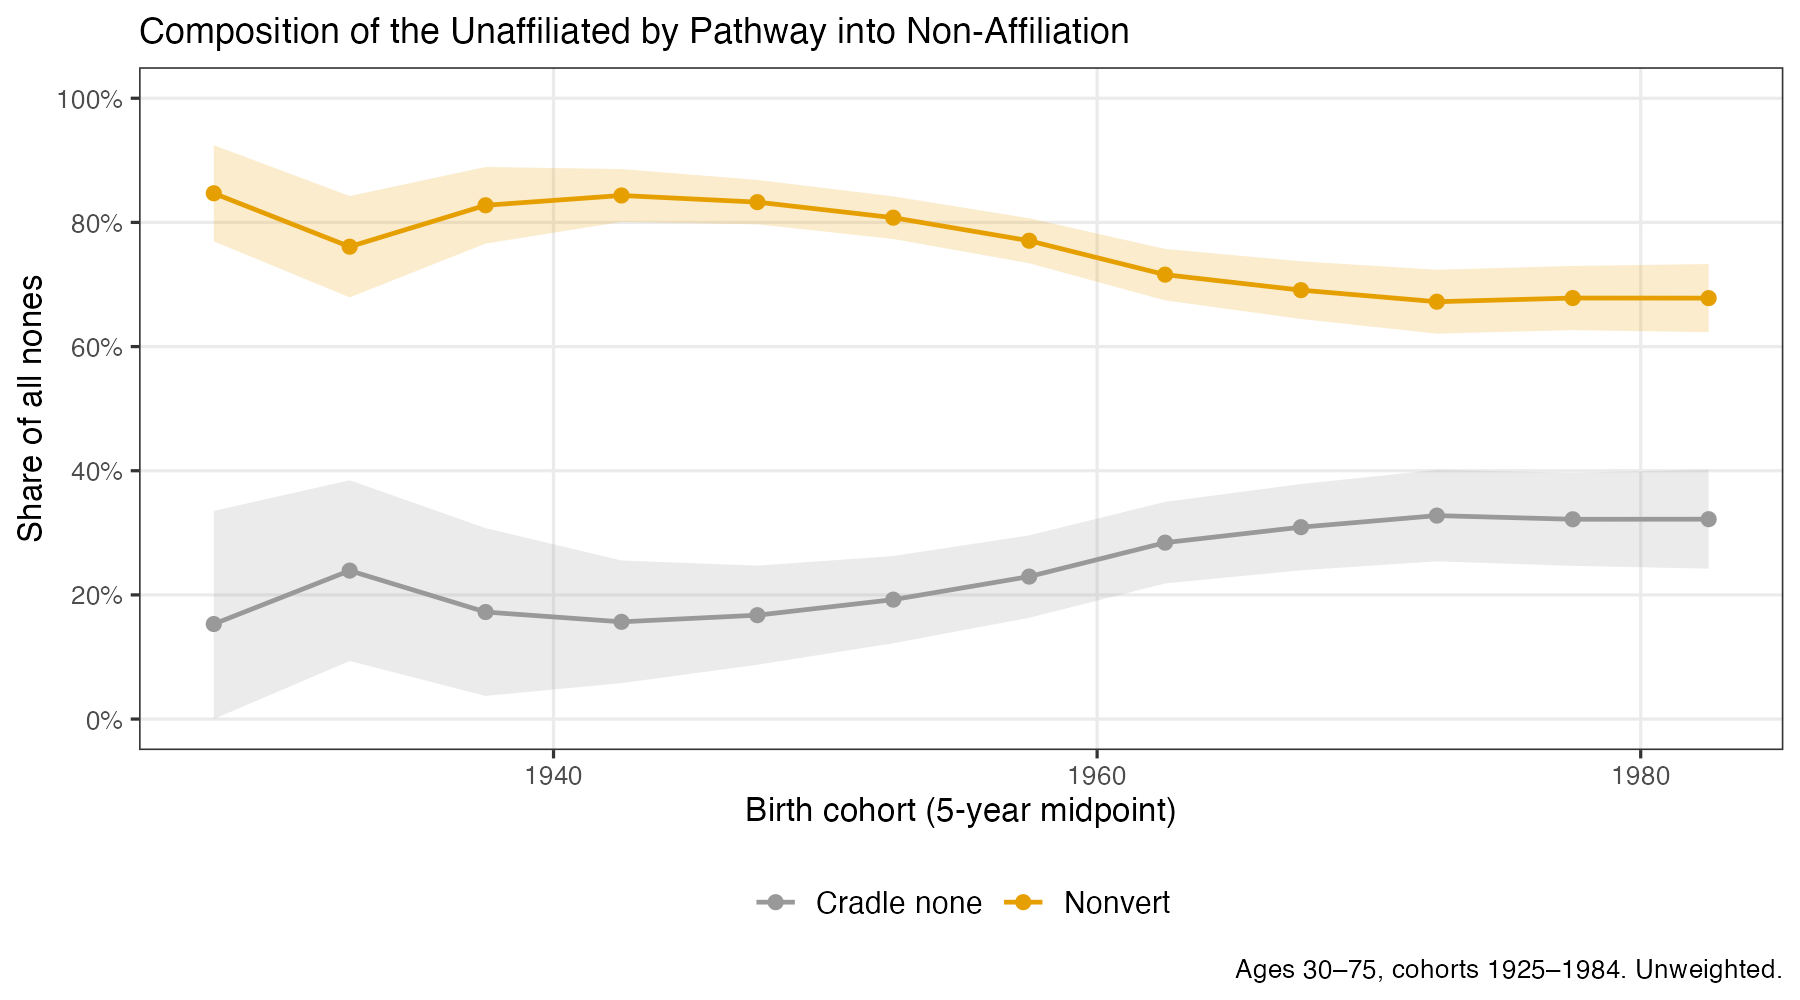
\includegraphics[width=\textwidth]{fig1_cradle_share.png}
  \caption{Share of currently unaffiliated respondents who are cradle nones
    (raised without religion) versus nonverts (adults who left a tradition),
    by 5-year birth cohort. Addresses whether growth in the unaffiliated
    reflects a secular-raised generation accumulating or continued defection
    from religious traditions.}
  \label{fig:cradle_share}
\end{figure}

\clearpage

\begin{figure}[htbp]
  \centering
  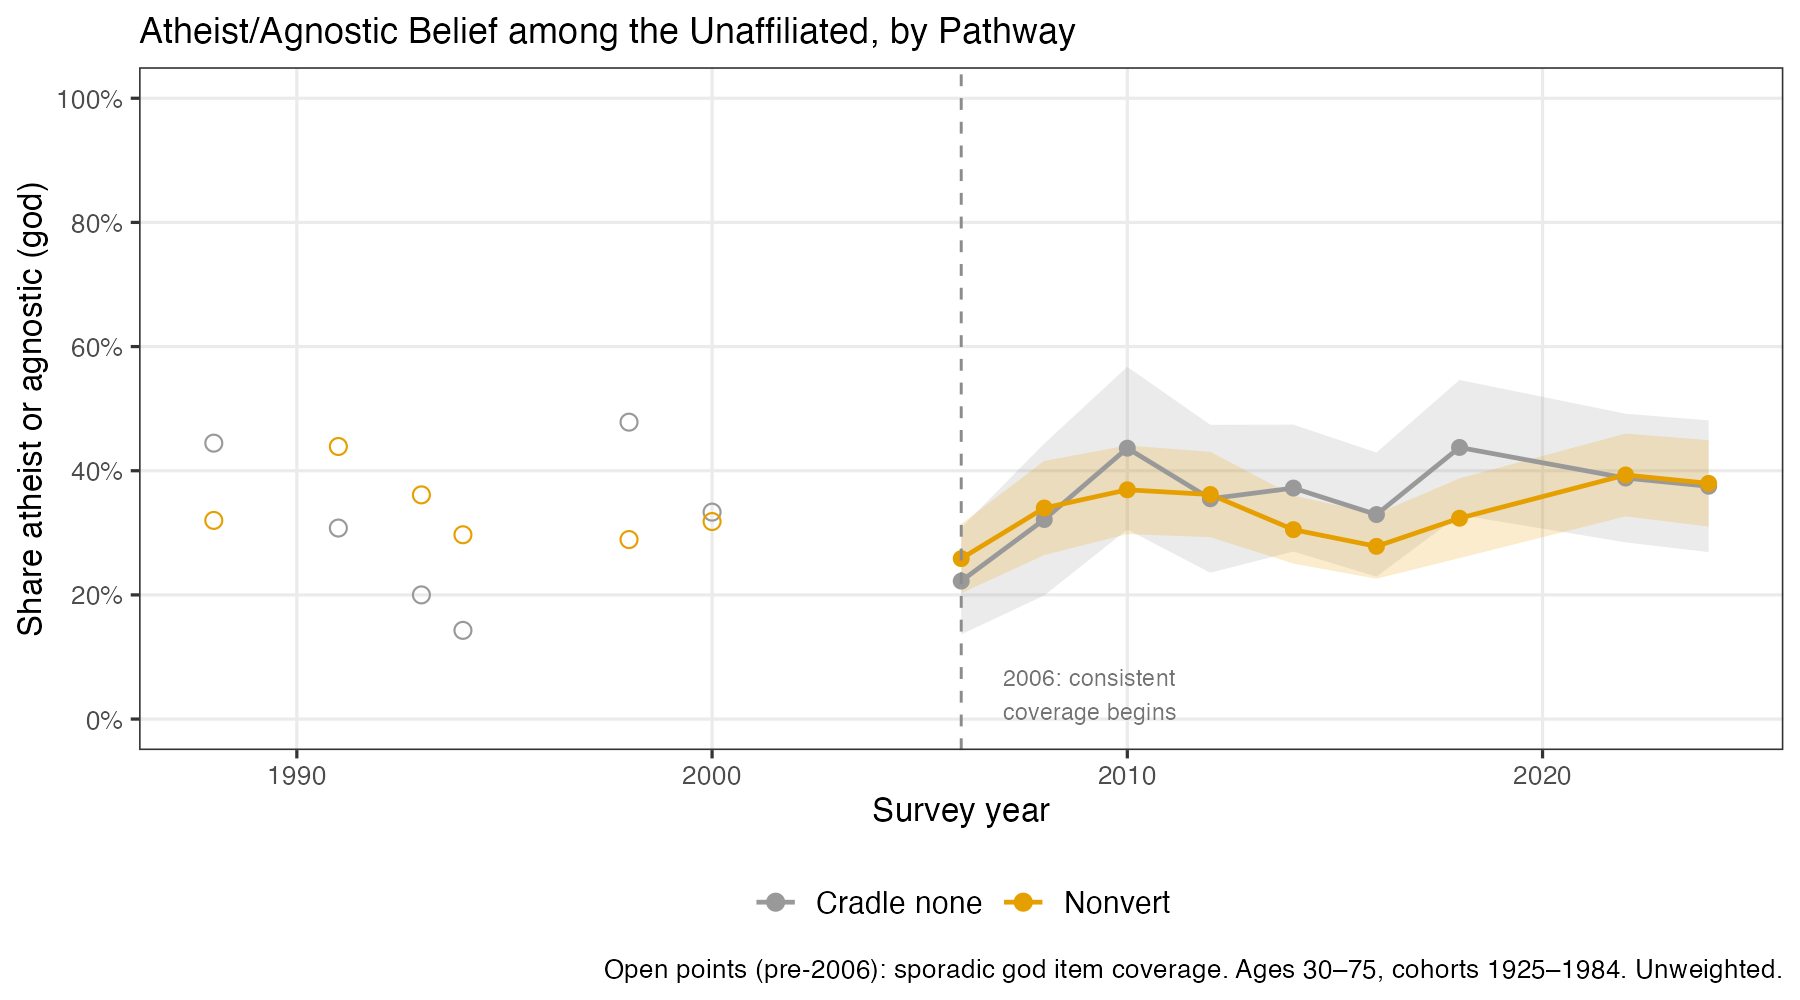
\includegraphics[width=\textwidth]{fig2_god_by_pathway.png}
  \caption{Share of unaffiliated respondents who are atheist or agnostic
    (\textit{god} scale, categories 1--2), by survey year and pathway (cradle
    none vs.\ nonvert). Addresses whether the two pathways are converging or
    diverging in explicit disbelief as non-affiliation has grown more common.
    Note: x-axis is survey year, not birth cohort, because \textit{god}-item
    coverage is too sparse before 2006 to support a cohort-based version.
    Open points (pre-2006) reflect sporadic item coverage.}
  \label{fig:god_by_pathway}
\end{figure}

\clearpage

\begin{figure}[htbp]
  \centering
  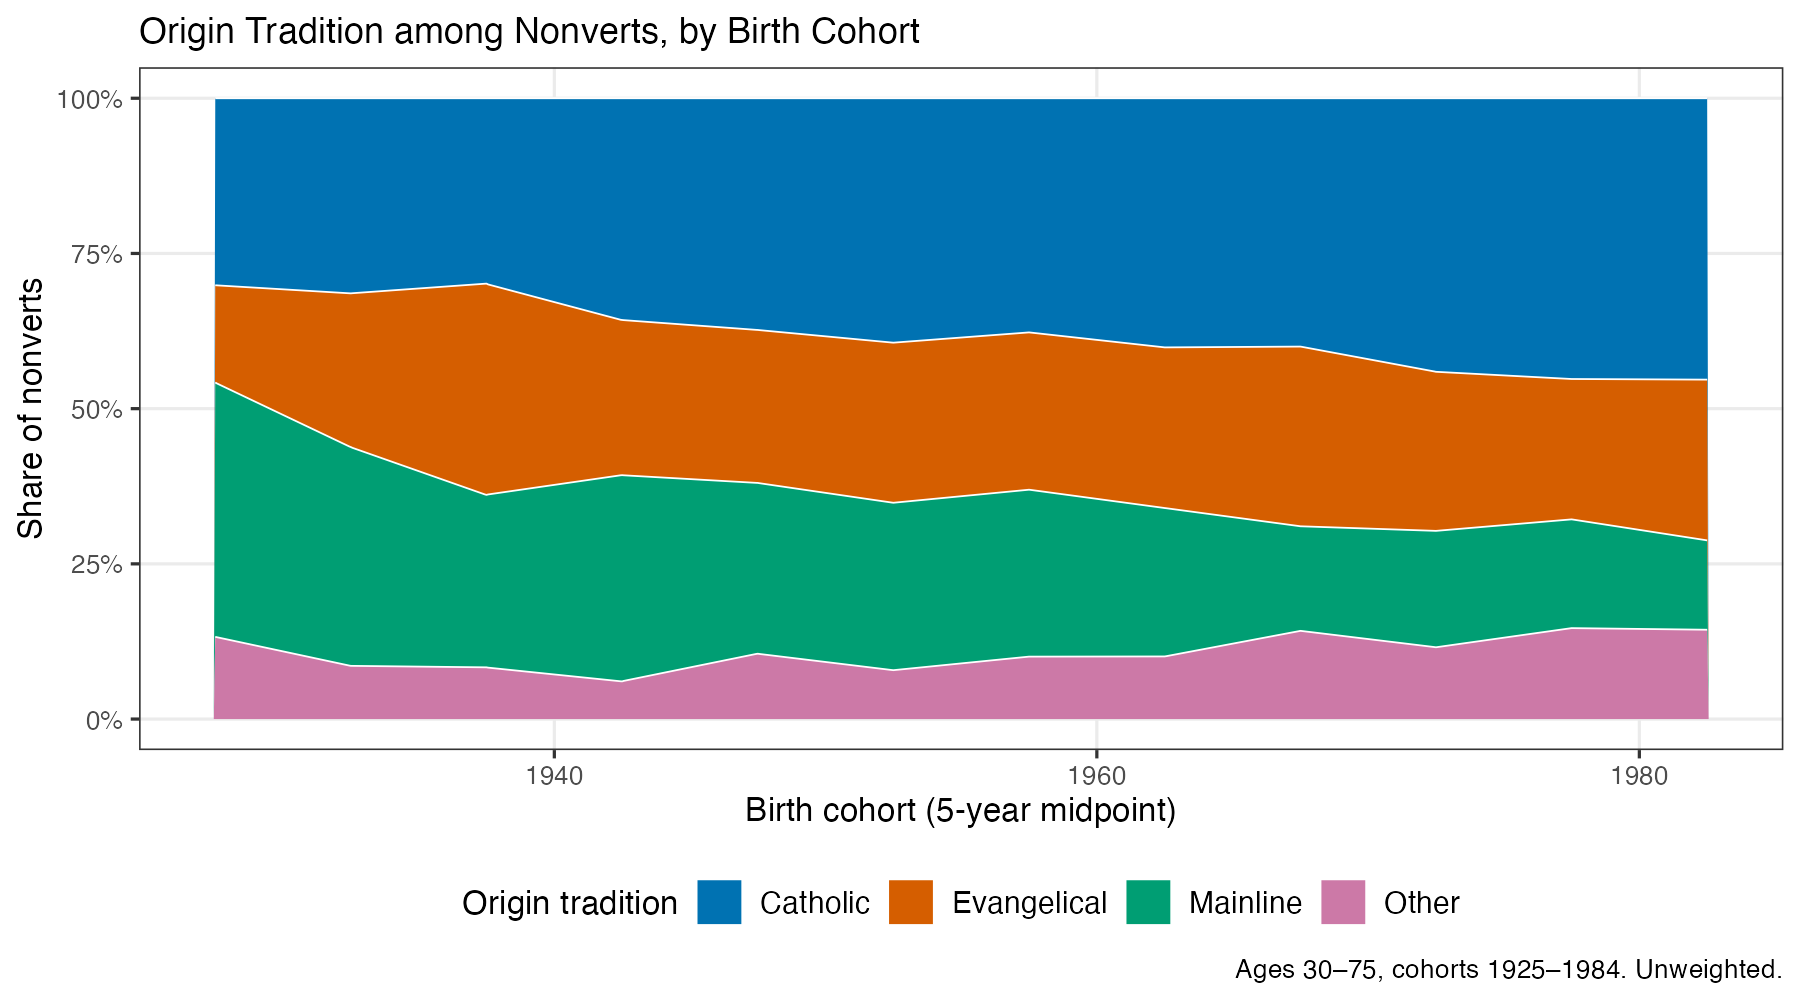
\includegraphics[width=\textwidth]{fig3_nonvert_origins.png}
  \caption{Origin tradition composition of nonverts (stacked area summing to
    100\%), by 5-year birth cohort. Addresses which traditions have been the
    primary source of defection for each cohort and whether the inflow
    structure has shifted over time.}
  \label{fig:nonvert_origins}
\end{figure}

\clearpage

\begin{figure}[htbp]
  \centering
  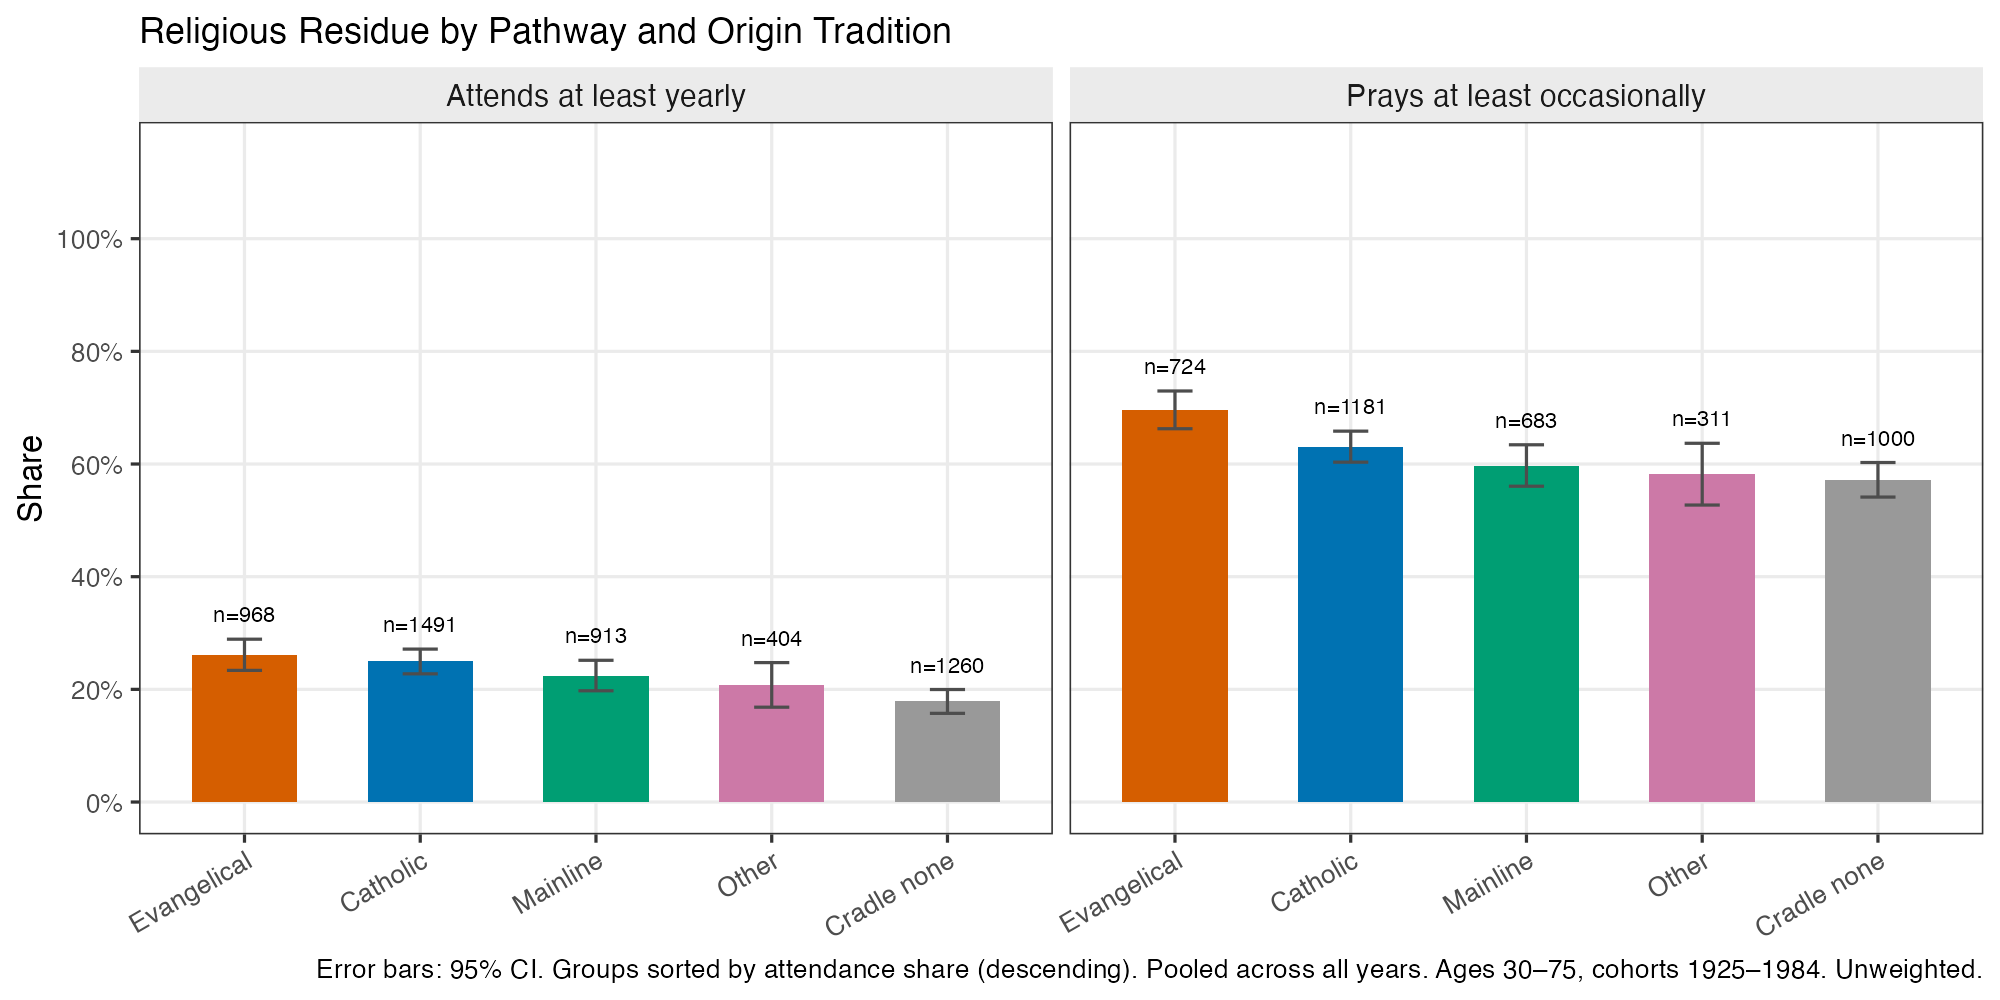
\includegraphics[width=\textwidth]{fig4_residue_gradient.png}
  \caption{Share attending religious services at least yearly (left panel) and
    praying at least occasionally (right panel), pooled across all survey
    years, for cradle nones and nonverts by origin tradition, sorted by
    attendance share. Error bars show 95\% confidence intervals. Addresses
    whether the tradition someone left predicts how much religious practice
    they retain (the religious-residue prediction).}
  \label{fig:residue_gradient}
\end{figure}

\clearpage

\begin{figure}[htbp]
  \centering
  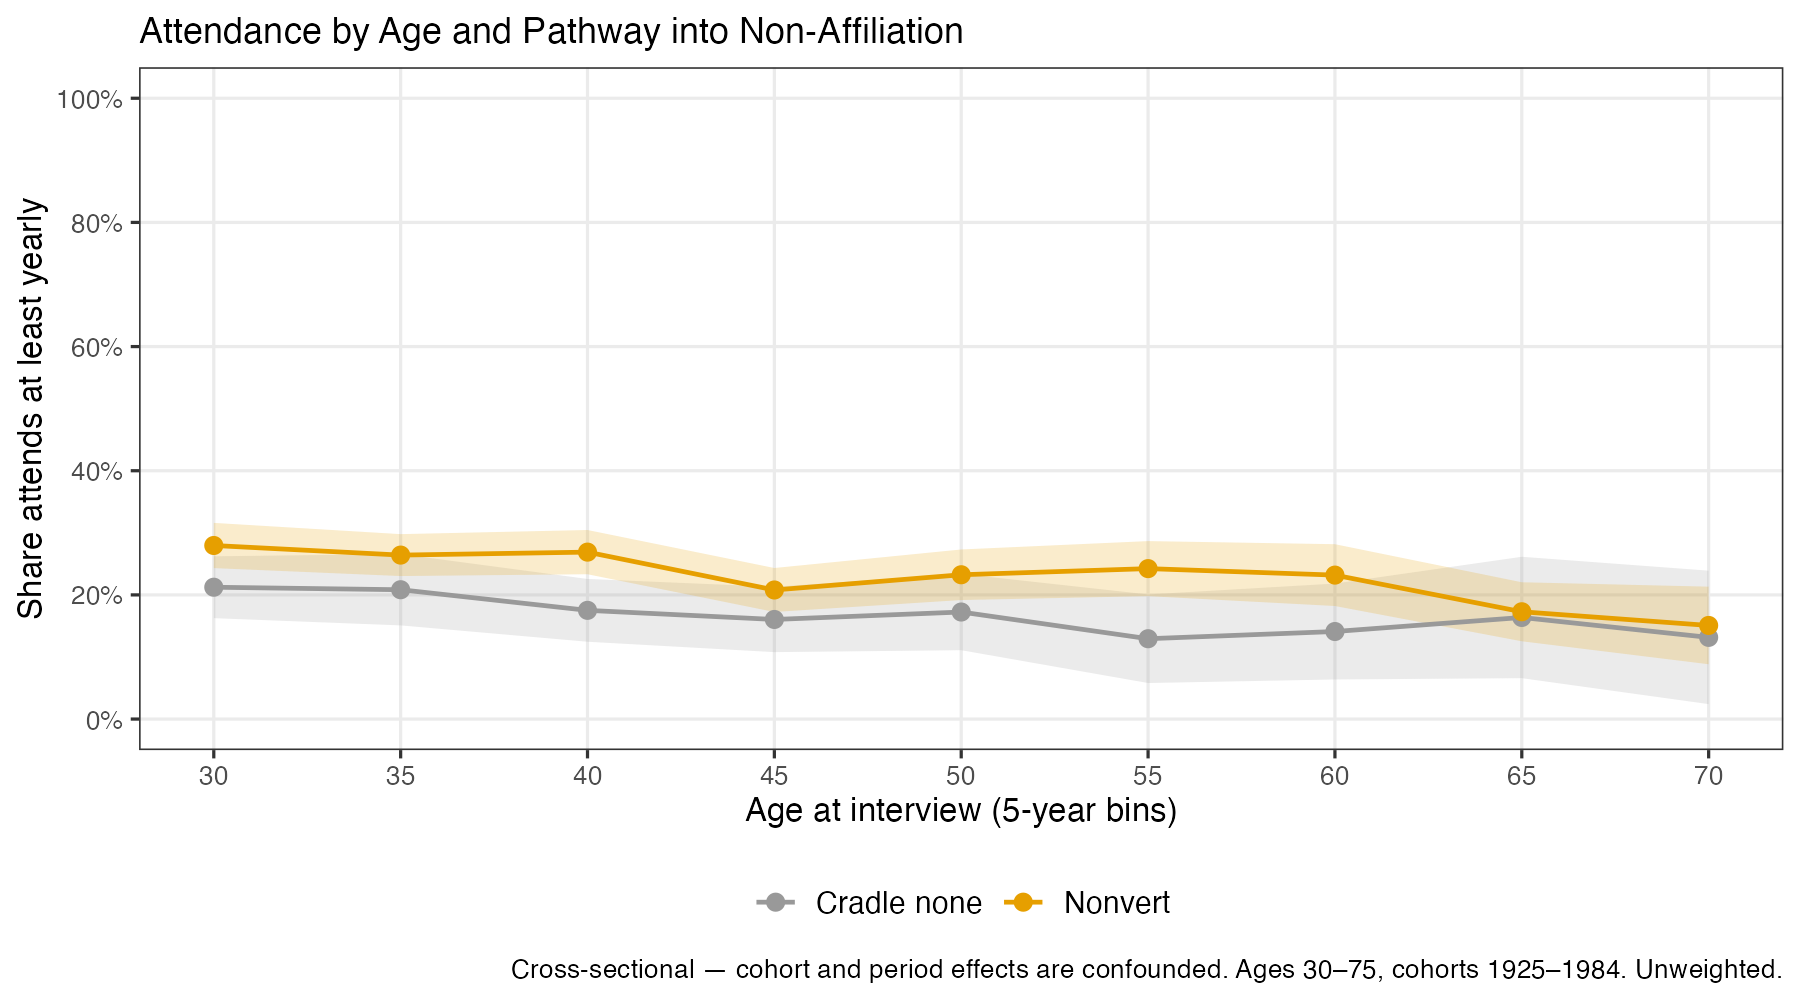
\includegraphics[width=\textwidth]{fig5_age_profile.png}
  \caption{Share attending religious services at least yearly by age at
    interview (5-year bins), separately for cradle nones and nonverts.
    Addresses whether the two pathways show different life-course attendance
    profiles; an age gradient among nonverts but not cradle nones would be
    consistent with liminality (a tradition to return to). Cross-sectional
    --- cohort and period effects are confounded.}
  \label{fig:age_profile}
\end{figure}

\end{document}
